\chapter{Methodology} \label{methodology}
Figure \ref{fig:method} represents the organisation and results for this research. The structure has been based on the findings of chapter \ref{relate}. This chapter will discuss, and expand upon the various steps. First block A, the description of the theoretical framework; followed by block B the evaluation of existing methods; concluding with block C the description and assessment of a proposed method. Some datasets and tools will be mentioned in this chapter, however a full overview of all proposed tools and datasets can be found in chapter \ref{tool}.

\begin{figure}[h]
	\centering
	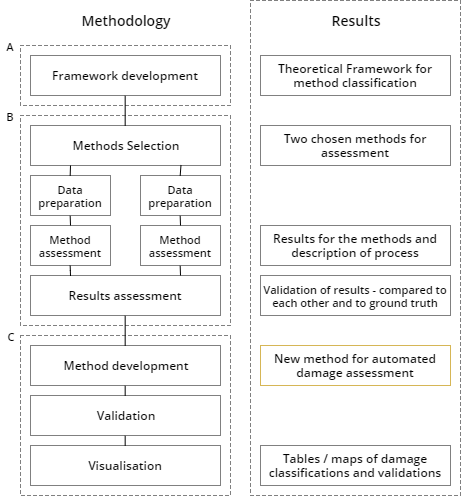
\includegraphics[width=0.9\textwidth]{figs/methodology.png}
	\caption{Methodology structure - the research objective is highlighted with a yellow boundary [From: own work]}
	\label{fig:method}
\end{figure}
\clearpage
\section{Theoretical framework}
For a solid basis, extensive literature research is required. The theoretical framework provides this comprehensive backing with the various criteria to which a method needs to suffice for efficient use in a disaster situation. The humanitarian field provides some of the criteria, besides those that are based on existing research for other methods. The combination of these allows for a new categorisation and overview of existing methods. \\
Besides the direct criteria for classification of methods, the theoretical framework also allows for background information on various topics needed in this methodology and to further define the scope for the research. 
Chapter \ref{relate} gives an overview of the developed framework, various criteria and background information.

\section {Existing methods} \label{emethod}
The extent of existing methods can be found in section \ref{sec:etech}. To reduce the scope of this research a selection out of this group will be made for further analysis. This investigation into these methods will serve as the base upon which the proposed method can be developed.\\
To adequately select methods for further assessment, the extensive group needs to be tested and classified based on the theoretical framework. The first selection is done on the results mentioned in the literature combined with the applicability in disaster situations. Methods are not excluded if they do damage assessment for other types of disasters as the indicators of damage are likely to correlate. The results of this selection can be found in section \ref{sec:smethod}.\\
Before the methods can be assessed, it is necessary to prepare the data. Normally this would involve the collection of data as well, however all data has already been collected in the response to Hurricane Irma from the \ac{nlrc}. An overview of the available datasets can be found in section \ref{sec:data}. These are however raw datasets and they need to be assessed and prepared before they can be used. An example of this is the productions of interferometric products using the tool Doris from the TU Delft \citep{Mgp}. An important preparation step for all datasets is the spatial matching and geo-referencing, however the topic of an automated approach can be a thesis on it's own and for this research a manual approach will be taken. A 30 meter resolution, \ac{dem} is available from \ac{jaxa} \citep{JAXA2017} to aid the correct matching of the datasets. \\
To better understand the existing methods for damage classification in disaster situations, the chosen methods will be prepared and executed for the case study area. These steps will provide insight in the transferability of existing methods to other disasters and provide benchmark results for automated classification. Techniques learned from the rebuilding of a method, preparation of data and subsequent results, could be transferred to the proposed method. The reconstruction of the existing methods will be done in software known and available to the author and will follow the described processes as closely as possible. \\
Since the result of a method is what will be needed by humanitarian organisations, it is necessary to validate and compare these. This comparison will be done between the results of the reconstructed methods and the ground truth generated by the \ac{nlrc}. This will be done in a one-to-one comparison as well as with deeper analysis. The latter will consist out of the analysis of variance of the classification and a confusion matrix as described in \citep{Antonietta2015}. Visualisation of the results is also part of the assessment. The outcomes of the methods and analysis need to be understood by those who have not been part of the whole process.\\

\section {Proposed method}
The development of a proposed method will focus on the fusion of characteristics of existing methods and datasets. Through the development of this proposed methods, the main research question will be answered. The synthesis of the best components of the previous assessed methods can lead to a more accurate, and effective approach to automated damage classification. In the process of development, the requirements towards data and tools will become clear. These might vary from those found in existing methods but will be based on similar principles.\\
The proposed method will not take into account the detection of buildings, as these are available from OpenStreetMap [\href{https://www.openstreetmap.org}{openstreetmap.org}] and have been updated shortly before the landfall of hurricane Irma on St. Maarten. These updates of the maps have been done by the volunteers of the Missing Maps network [\href{https://www.missingmaps.org}{missingmaps.org}] and are validated by experienced cartographers. \\
Validation of the method will assess the accuracy and effectiveness. These will be compared to the outcomes of the assessment of existing methods. Similar analysis will be used on the results as described in section \ref{emethod}. The method will also be tested on the theoretical framework, which has been used for the selection of the existing models.\\
From all the development of the method and subsequent analysis various results will be visualised for a more accessible transfer of knowledge. The goal of the proposed method would be an accurate classification of the damage on a building level visualised on a map. These could be aggregated to higher levels, e.g. block or neighbourhood level, for other uses in the field. The results of the analysis of the methods will be more statistical and will need to be summarised in tables and percentiles.\\

